Seja a função potencial
\begin{equation}
	U(x) =
	\begin{cases}
		0,    & \mbox{se}\; -\infty<x<-L/2      \\
		-V_0, & \mbox{se}\; -L/2 \le x \le +L/2 \\
		0,    & \mbox{se}\; +L/2<x<\infty       \\
	\end{cases}\;.
\end{equation}

Seja a equação de Schrödinger unidimensional

\begin{equation}
	\frac{d^2\,\psi(x)}{dx^2} = \frac{2\,m}{\hbar^2}\;(U(x)-E)\;\psi(x)
\end{equation}

\noindent Conforme enunciado na questão, a partícula está confinada no poço de
potencial. Portanto, $E<0$.

OBS: Em ordem de simplificar os cálculos, a substituição $a=L/2$ será
utilizada.

Nas regiões I ($-\infty<x<-a$) e III ($+a<x<\infty$), tem-se

\begin{equation}
	\begin{array}{lcl}
		\frac{d^2\,\psi(x)}{dx^2} & = & \frac{-2\,m\,E}{\hbar^2}\;\psi(x) \\
		                          & = & \alpha^{2}\;\psi(x)
	\end{array}\;,
\end{equation}

\noindent onde $\alpha = \sqrt{-2\,m\,E}/\hbar$. E na região II ($-a \le x \le
	+a$),

\begin{equation}
	\begin{array}{lcl}
		\frac{d^2\,\psi(x)}{dx^2} & = & -\frac{2\,m}{\hbar^2}\;(E+V_0)\;\psi(x) \\
		                          & = & -k^{2}\;\psi(x)                         \\
	\end{array}\;,
\end{equation}

\noindent onde $k = \sqrt{2\,m\,(E+V_0)}/\hbar$.

Assim, as soluções das EDOs nas regiões I, II e III terão, respectivamente, os
seguintes formatos

\begin{equation}
	\psi(x) =
	\begin{cases}
		\psi_{1}(x) = A_1\,e^{i\,\alpha\,x} + B_1\,e^{-i\,\alpha\,x},
		 & \mbox{se}\;x<-a    \\
		\psi_{2}(x) = A_2\,sen(k\,x) + B_2\,cos(k\,x),
		 & \mbox{se}\;-a<x<+a \\
		\psi_{3}(x) = A_3\,e^{i\,\alpha\,x} + B_3\,e^{-i\,\alpha\,x},
		 & \mbox{se}\;x>+a
	\end{cases}\;.
\end{equation}

\noindent Uma vez que $B_1$ e $A_3$ precisam ser nulos para que não haja
divergência, tem-se:

\begin{equation}
	\psi(x) =
	\begin{cases}
		\psi_{1}(x) = A_1\,e^{i\,\alpha\,x},
		 & \mbox{se}\;x<-a    \\
		\psi_{2}(x) = A_2\,sen(k\,x) + B_2\,cos(k\,x),
		 & \mbox{se}\;-a<x<+a \\
		\psi_{3}(x) = B_3\,e^{-i\,\alpha\,x},
		 & \mbox{se}\;x>+a
	\end{cases}\;.
\end{equation}

Como pode ser observado, o problema é simétrico em $x$ e, portanto, pode ser
solucionado a partir da análise das condições de continuidade
e diferenciabilidade em apenas uma das fronteiras.

Tomando a interface entre as regiões I e II ($x=-a$), são desenvolvidos os
sitemas refrenrentes às soluções par e ímpar, respectivamente:

\begin{equation}
	\mbox{Sol. Par}
	\begin{cases}
		A_1\,e^{-\alpha\,a} = B_2\,cos(-k\,a) \\
		\alpha\,A_1\,e^{-\alpha\,a} = -k\,B_2\,sen(-k\,a)
	\end{cases}
	\mbox{Sol. Ímpar}
	\begin{cases}
		A_1\,e^{-\alpha\,a} = A_2\,sen(-k\,a) \\
		\alpha\,A_1\,e^{-\alpha\,a} = k\,A_2\,cos(-k\,a)
	\end{cases}
\end{equation}

\noindent Aplicando uma divisão direta entre as equações em cada sistema,
encontra-se

\begin{equation}
	\begin{array}{lcl}
		\alpha    & = & k\,tan(k\,a)    \\
		\alpha\,a & = & k\,a\,tan(k\,a)
	\end{array}
\end{equation}

\noindent e

\begin{equation}
	\begin{array}{lcl}
		\alpha    & = & -k\,cotg(k\,a)    \\
		\alpha\,a & = & -k\,a\,cotg(k\,a)
	\end{array}
\end{equation}

\noindent Seja

\begin{equation}
	(k\,a)^2 + (\alpha\,a)^2 = \frac{2\,m\,V_0\,a^2}{\hbar^2}\;,
\end{equation}

\noindent por conveniência, aplicam-se as seguintes substituições:

\begin{equation}
	\begin{cases}
		X     & = k\,a                           \\
		Y     & = \alpha\,a                      \\
		R_0^2 & = \frac{2\,m\,V_0\,a^2}{\hbar^2}
	\end{cases}
\end{equation}

Deste modo, reescrevendo os sistemas para as soluções par e ímpar, obtém-se

\begin{equation}
	\mbox{Sol. Par}
	\begin{cases}
		Y = X\,tan(X) \\
		Y = \sqrt{R_0^2 - X^2}
	\end{cases}
	\mbox{Sol. ímpar}
	\begin{cases}
		Y = -X\,cotg(X) \\
		Y = \sqrt{R_0^2 - X^2}
	\end{cases}
\end{equation}

Dado que $-V_0<E<0$, tem-se que o maior e o menor valor que X pode assumir são,
respectivamente,

\begin{equation}
	X(E=0) = k(E=0)\,a = \frac{\sqrt{2\,m\,(0+V_0)}}{\hbar}\,a
	= \frac{\sqrt{2\,m\,V_0}}{\hbar}\,a = R_0
\end{equation}

\begin{equation}
	X(E=-V_0) = k(E=-V_0)\,a = \frac{\sqrt{2\,m\,(-V_0+V_0)}}{\hbar}\,a = 0
\end{equation}

Com isto, conclui-se que os estados possíveis de energia da partícula podem ser
encontrados por meio das intersecções entre as curvas dos sistemas das
soluções par e ímpar:

\begin{equation}
	\mbox{Sol. Par: }\;\left( X\,tan(X)=\sqrt{R_0^2-X^2},\;\mbox{onde
	}\,0<X<R_0 \right)
\end{equation}

\begin{equation}
	\mbox{Sol. Ímpar: }\;\left( -X\,cotg(X)=\sqrt{R_0^2-X^2},\;\mbox{onde
	}\,0<X<R_0 \right)
\end{equation}

\begin{figure}[H] \centering
	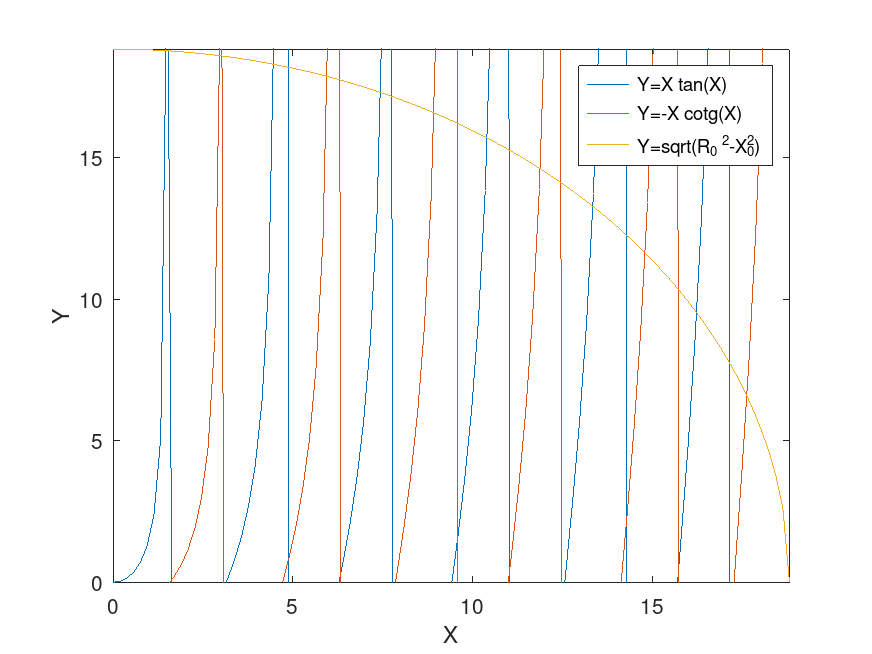
\includegraphics[width=1\textwidth]{../images/q3a.png}
	\caption{ Interseções que representam os níveis possíveis de energia da
		partícula confinada }
	\label{fig:q3a}
\end{figure}

Coletando os valores diretamente do gráfico, tem-se que

\begin{equation}
	\begin{cases}
		X_{1,par}   & = 1.46  \\
		X_{2,par}   & = 4.44  \\
		X_{3,par}   & = 7.42  \\
		X_{4,par}   & = 10.40 \\
		X_{5,par}   & = 13.35 \\
		X_{6,par}   & = 16.23 \\
		X_{1,impar} & = 2.95  \\
		X_{2,impar} & = 5.94  \\
		X_{3,impar} & = 8.91  \\
		X_{4,impar} & = 11.88 \\
		X_{5,impar} & = 14.80 \\
		X_{6,impar} & = 17.63 \\
	\end{cases}
\end{equation}

\noindent Convertendo para valores de energia, tem-se

\begin{equation}
	\begin{cases}
		E_{1}  & = -2.3888\;10^{-20} [J] \\
		E_{2}  & = -2.3443\;10^{-20} [J] \\
		E_{3}  & = -2.2696\;10^{-20} [J] \\
		E_{4}  & = -2.1640\;10^{-20} [J] \\
		E_{5}  & = -2.0299\;10^{-20} [J] \\
		E_{6}  & = -1.8648\;10^{-20} [J] \\
		E_{7}  & = -1.6697\;10^{-20} [J] \\
		E_{8}  & = -1.4460\;10^{-20} [J] \\
		E_{9}  & = -1.1945\;10^{-20} [J] \\
		E_{10} & = -9.1760\;10^{-21} [J] \\
		E_{11} & = -6.1662\;10^{-21} [J] \\
		E_{12} & = -2.9509\;10^{-21} [J] \\
	\end{cases}
\end{equation}

Dado que $Y=\sqrt{R_0^2-X^2}$ em $0<X<R_0$ é um quadrante de circunferência
e que $Y=X\,tan(X)$ terá apenas alguns pontos de intersecção com este círculo,
pode-se obter o número de soluções possíveis para E através das seguintes
equações:

\begin{equation}
	N_{par} = floor\left(\frac{R_0}{\pi}\right)+1
\end{equation}

\begin{equation}
	N_{impar} = floor\left(\frac{R_0 + \frac{\pi}{2} }{\pi}\right)
\end{equation}

\begin{equation}
	N_{total} = N_{par} + N_{impar}
	= floor\left(\frac{\sqrt{2\,m\,V_0}\,a}{\hbar\,\pi}\right)
	+ floor\left(\frac{\sqrt{2\,m\,V_0}\,a}{\hbar\,\pi} + 0.5\right) + 1
\end{equation}

Em ordem de calcular a probabilidade de se encontrar a partícula fora da região
do poço de potencial é necessário obter os valores de $A_1$, $A_2$, $B_2$
e $B_3$ nos diferentes níveis de $E_n$.
